%%%%%%%%%%%%%%%%%%%%%%%%%%%%%%%%%%%%%%%%%%%%%%%%%%%%%%%%%%%%%%%%%%%%%
% PREAMBLE
%%%%%%%%%%%%%%%%%%%%%%%%%%%%%%%%%%%%%%%%%%%%%%%%%%%%%%%%%%%%%%%%%%%%%
%
% The following two commands will generate a PDF that follows all the requirements for submission
% and peer review.  Uncomment these commands to generate this output (and comment out the two lines below.)
%
% DOUBLE SPACE VERSION FOR SUBMISSION TO THE AMS
\documentclass[11pt]{article}
\usepackage{ametsoc}
% \usepackage{ametsoc2col}
%\linenumbers
\graphicspath{{/Users/jklymak/PW13/figs/mvp/}}
\usepackage[plain]{fancyref}
\usepackage{xcolor}
\usepackage{lineno}
\newcommand{\tempS}[1]{}
\newcommand{\twowidth}[0]{6.4in}
\newcommand{\onewidth}[0]{3.2in}
\newcommand{\mn}[1]{{\sc #1}}
\DeclareGraphicsExtensions{%
    .pdf,.png}
%
% The following two commands will generate a single space, double column paper that closely
% matches an AMS journal page.  Uncomment these commands to generate this output (and comment
% out the two lines above. FOR AUTHOR USE ONLY. PAPERS SUBMITTED IN THIS FORMAT WILL BE RETURNED
% TO THE AUTHOR for submission with the correct formatting.
%
% TWO COLUMN JOURNAL PAGE LAYOUT FOR AUTHOR USE ONLY
%%%%\documentclass[10pt]{article}
%%%%\usepackage{ametsoc2col}
%
%%%%%%%%%%%%%%%%%%%%%%%%%%%%%%%%%%%%%%%%%%%%%%%%%%%%%%%%%%%%%%%%%%%%%
% ABSTRACT
%
% Enter your Abstract here
%%%%%%%%%%%%%%%%%%%%%%%%%%%%%%%%%%%%%%%%%%%%%%%%%%%%%%%%%%%%%%%%%%%%%
\linenumbers
\newcommand{\myabstract}{}
%
\begin{document}
%
%%%%%%%%%%%%%%%%%%%%%%%%%%%%%%%%%%%%%%%%%%%%%%%%%%%%%%%%%%%%%%%%%%%%%
% TITLE
%
% Enter your TITLE here
%%%%%%%%%%%%%%%%%%%%%%%%%%%%%%%%%%%%%%%%%%%%%%%%%%%%%%%%%%%%%%%%%%%%%
\title{\textbf{\large{Evidence for cross-shelf exchange driven by a submarine canyon}}}
%
% Author names, with corresponding author information.
% [Update and move the \thanks{...} block as appropriate.]
%
\author{\textsc{Jody M. Klymak,}
				\thanks{\textit{Corresponding author address:}
				Jody Klymak, University of Victoria, Victoria, BC, Canada
				\newline{E-mail: jklymak@uvic.ca}}\quad
				\\
\textit{\footnotesize{School of Earth and Ocean Sciences and Department of Physics and Astronomy, University of Victoria, Victoria, Canada}}
}
%
% Formatting done here...Authors should skip over this.  See above for abstract.
\ifthenelse{\boolean{dc}}
{
\twocolumn[
\begin{@twocolumnfalse}
\amstitle

% Start Abstract (Enter your Abstract above.  Do not enter any text here)
\begin{center}
\begin{minipage}{13.0cm}
\begin{abstract}
	\myabstract
	\newline
	\begin{center}
		\rule{38mm}{0.2mm}
	\end{center}
\end{abstract}
\end{minipage}
\end{center}
\end{@twocolumnfalse}
]
}
{
\amstitle
\begin{abstract}
\myabstract
\end{abstract}
\newpage
}
%%%%%%%%%%%%%%%%%%%%%%%%%%%%%%%%%%%%%%%%%%%%%%%%%%%%%%%%%%%%%%%%%%%%%
% MAIN BODY OF PAPER
%%%%%%%%%%%%%%%%%%%%%%%%%%%%%%%%%%%%%%%%%%%%%%%%%%%%%%%%%%%%%%%%%%%%%
\section{Introduction}

Cross-shelf exchange is important to the health and productivity of continental shelf regions, where offshore nutrients and oxygenated water is exchanged with nutrient and oxygen depleted near-shore water.  Cross-shelf transport requires a level of ageostrophic flow since balanced flow will tend to follow topographic contours, often providing a barrier to lateral exchange.  Mechanisms for cross-shelf exchange include internal waves and instabilities in shelf-break fronts.  Most-dramatically, however, topography can drive cross-slope exchanges, often seen most clearly in surface



%\citet{klymaketal10a}

\section{Site and Methods}
\label{sec:Site}

Data collection was between 21 and 30 August, 2013, aboard the \emph{R/V Falkor}.  The study site was the southern portion of the Vancouver Island Shelf (\fref{fig:LocMapBoth}a), a particularly complicated region due to the bathymetry and varied forcing.

\begin{figure*}[htbp]
  \begin{center}

     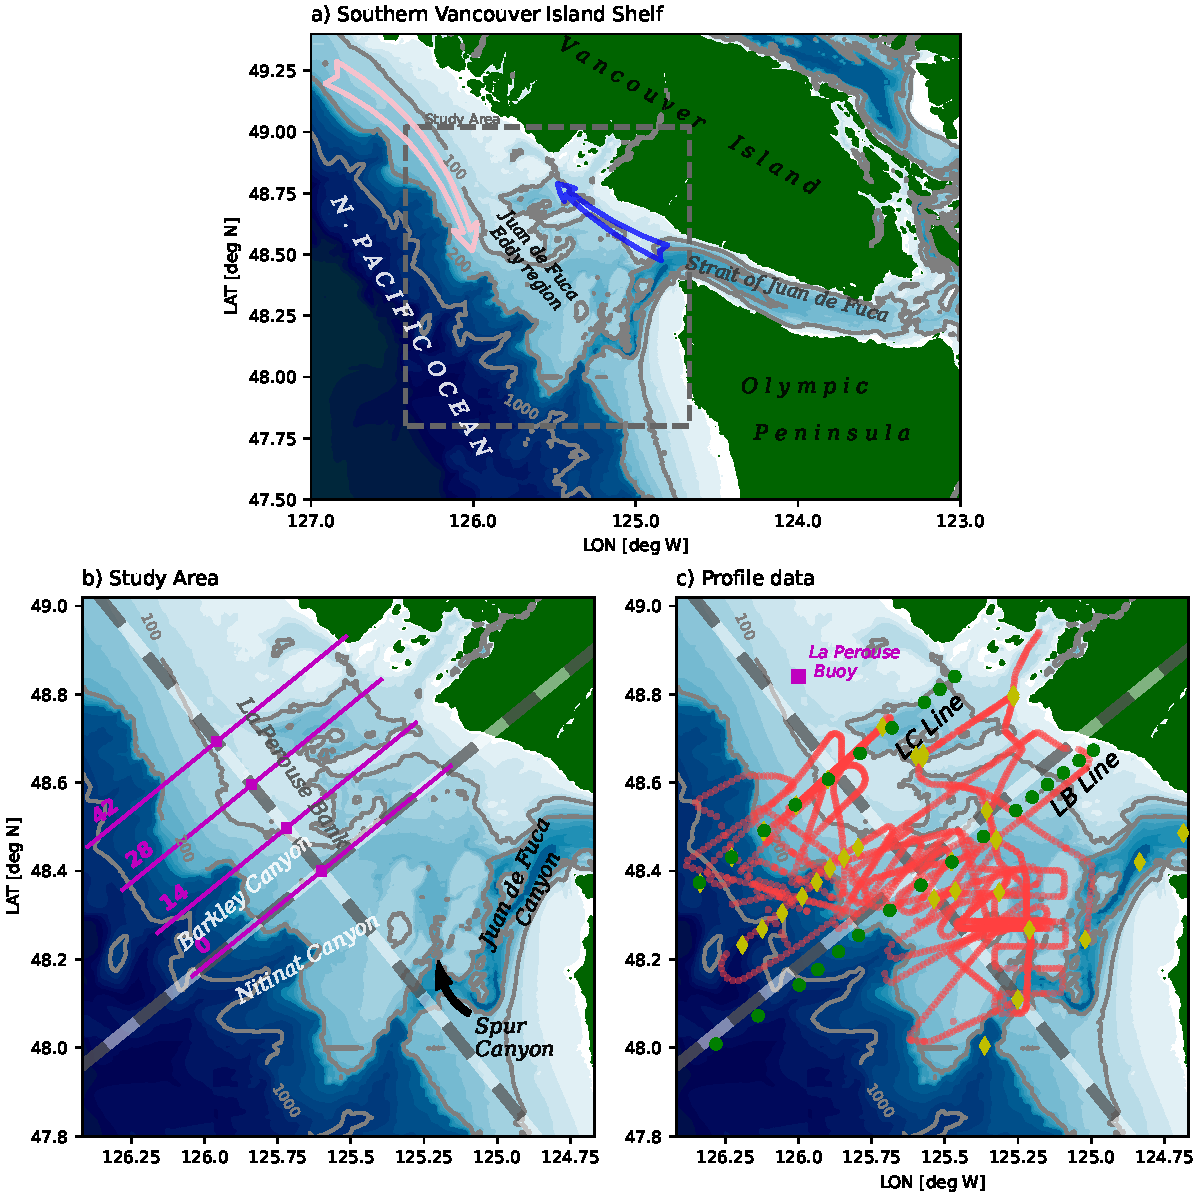
\includegraphics[width=6.2in]{LocMapBoth.pdf}
    \caption{a) Study site on the Vancouver Island Shelf.  The blue arrow indicates the direction of the Vancouver Island Current.  The pink arrow indicates southward flow of the coastal upwelling current.  The dashed box indicates the approximate limits of the study area.  b) The study area with standard hydrographic casts indicated in yellow dots, and Moving Vessel Profiler casts as red dots.
      \tempS{\footnotesize /Users/jklymak/PW13/figs/mvp///MvpProc.ipynb ;
        /Users/jklymak/PW13/figs/mvp//LocMapBoth.pdf}
      \label{fig:LocMapBoth} }
  \end{center}
\end{figure*}

\begin{figure*}[htbp]
  \begin{center}
    \includegraphics[width=6.2in]{SpiceO2264}
    \caption{Spatial overview of a) local spice (temperature anomaly on an isopycnal: see text), and b) oxygen saturation on the $\sigma_{\theta} = 26.4\ \mathrm{kg\,m^{-3}}$ isopycnal.  Grey cross-slope lines are cross sections indicated in \fref{fig:CrossSectionsSpice}.  Along-slope grey lines are every 20 km in the cross-slope direction, with $x=0\ \mathrm{km}$ near the 100-m isobath at the north end of the observation area.

      \tempS{\footnotesize /Users/jklymak/PW13/figs/mvp///MvpProcNew.ipynb ;
        /Users/jklymak/PW13/figs/mvp//SpiceO2264.pdf}
      \label{fig:SpiceO2264} }
  \end{center}
\end{figure*}

\begin{figure*}[htbp]
  \begin{center}
    \includegraphics[width=6.2in]{CrossSectionsSpice}
    \caption{
      \tempS{\footnotesize /Users/jklymak/PW13/figs/mvp///MvpProcNew.ipynb ;
        /Users/jklymak/PW13/figs/mvp//CrossSectionsSpice.pdf}
      \label{fig:CrossSectionsSpice} }
  \end{center}
\end{figure*}

\begin{figure}[htbp]
  \begin{center}
    \includegraphics[width=3in]{TsLineDefn}
    \caption{
      \tempS{\footnotesize /Users/jklymak/PW13/figs/mvp///MvpProcNew ;
        /Users/jklymak/PW13/figs/mvp//TsLineDefn.pdf}
      \label{fig:TsLineDefn} }
  \end{center}
\end{figure}


%\begin{appendix}


%\subsection{First appendix secondary heading}
%
%\subsection{Second appendix secondary heading}
%
%\subsubsection{First appendix tertiary heading}
%
%\subsubsection{Second appendix tertiary heading}
%
%\paragraph{First appendix quaternary heading}
%
%\paragraph{Second appendix quaternary heading}
%
%\end{appendix}

% Create a bibliography directory and place your .bib file there.
% -REMOVE ALL DIRECTORY PATHS TO REFERENCE FILES BEFORE SUBMITTING TO THE AMS FOR PEER REVIEW
\ifthenelse{\boolean{dc}}
{}
{\clearpage}
\bibliographystyle{ametsocjmk}
\bibliography{main}

%%%%%%%%%%%%%%%%%%%%%%%%%%%%%%%%%%%%%%%%%%%%%%%%%%%%%%%%%%%%%%%%%%%%%
% FIGURES-REMOVE ALL DIRECTORY PATHS TO FIGURE FILES BEFORE SUBMITTING TO THE AMS FOR PEER REVIEW
%%%%%%%%%%%%%%%%%%%%%%%%%%%%%%%%%%%%%%%%%%%%%%%%%%%%%%%%%%%%%%%%%%%%%

%
\end{document}
